%%%%%%%%%%%%%%%%%%%%%%%%%%%%%%
%%% Compile with LuaLaTeX! %%%
%%%%%%%%%%%%%%%%%%%%%%%%%%%%%%

% This must be in the first 5 lines to tell arXiv to use pdfLaTeX, which is strongly recommended.
% \pdfoutput=1
% In particular, the hyperref package requires pdfLaTeX in order to break URLs across lines.

\documentclass[11pt]{article}

% Change "review" to "final" to generate the final (sometimes called camera-ready) version.
% Change to "preprint" to generate a non-anonymous version with page numbers.
\usepackage[review]{acl}

% Standard package includes
% \usepackage{times}
% \usepackage{latexsym}

% For proper rendering and hyphenation of words containing Latin characters (including in bib files)
% \usepackage[T1]{fontenc}
% For Vietnamese characters
% \usepackage[T5]{fontenc}
% See https://www.latex-project.org/help/documentation/encguide.pdf for other character sets

% This assumes your files are encoded as UTF8
% \usepackage[utf8]{inputenc}

% This is not strictly necessary, and may be commented out,
% but it will improve the layout of the manuscript,
% and will typically save some space.
\usepackage{microtype}

% This is also not strictly necessary, and may be commented out.
% However, it will improve the aesthetics of text in
% the typewriter font.
\usepackage{inconsolata}

%Including images in your LaTeX document requires adding
%additional package(s)
\usepackage{graphicx}

% Custom packages
% \usepackage{lmodern}
\usepackage{fontspec}
\setmainfont{Times New Roman}
\usepackage{csquotes}
\usepackage{hyperref}
\usepackage{soul}

% If the title and author information does not fit in the area allocated, uncomment the following
%
%\setlength\titlebox{<dim>}
%
% and set <dim> to something 5cm or larger.

\title{Occupational gender bias in ungendered languages: Comparing experimental data from Hungarian and Chinese}

% Author information can be set in various styles:
% For several authors from the same institution:
% \author{Author 1 \and ... \and Author n \\
%         Address line \\ ... \\ Address line}
% if the names do not fit well on one line use
%         Author 1 \\ {\bf Author 2} \\ ... \\ {\bf Author n} \\
% For authors from different institutions:
% \author{Author 1 \\ Address line \\  ... \\ Address line
%         \And  ... \And
%         Author n \\ Address line \\ ... \\ Address line}
% To start a separate ``row'' of authors use \AND, as in
% \author{Author 1 \\ Address line \\  ... \\ Address line
%         \AND
%         Author 2 \\ Address line \\ ... \\ Address line \And
%         Author 3 \\ Address line \\ ... \\ Address line}

\author{First Author \\
  Affiliation / Address line 1 \\
  Affiliation / Address line 2 \\
  Affiliation / Address line 3 \\
  \texttt{email@domain} \\\And
  Second Author \\
  Affiliation / Address line 1 \\
  Affiliation / Address line 2 \\
  Affiliation / Address line 3 \\
  \texttt{email@domain} \\}

%\author{
%  \textbf{First Author\textsuperscript{1}},
%  \textbf{Second Author\textsuperscript{1,2}},
%  \textbf{Third T. Author\textsuperscript{1}},
%  \textbf{Fourth Author\textsuperscript{1}},
%\\
%  \textbf{Fifth Author\textsuperscript{1,2}},
%  \textbf{Sixth Author\textsuperscript{1}},
%  \textbf{Seventh Author\textsuperscript{1}},
%  \textbf{Eighth Author \textsuperscript{1,2,3,4}},
%\\
%  \textbf{Ninth Author\textsuperscript{1}},
%  \textbf{Tenth Author\textsuperscript{1}},
%  \textbf{Eleventh E. Author\textsuperscript{1,2,3,4,5}},
%  \textbf{Twelfth Author\textsuperscript{1}},
%\\
%  \textbf{Thirteenth Author\textsuperscript{3}},
%  \textbf{Fourteenth F. Author\textsuperscript{2,4}},
%  \textbf{Fifteenth Author\textsuperscript{1}},
%  \textbf{Sixteenth Author\textsuperscript{1}},
%\\
%  \textbf{Seventeenth S. Author\textsuperscript{4,5}},
%  \textbf{Eighteenth Author\textsuperscript{3,4}},
%  \textbf{Nineteenth N. Author\textsuperscript{2,5}},
%  \textbf{Twentieth Author\textsuperscript{1}}
%\\
%\\
%  \textsuperscript{1}Affiliation 1,
%  \textsuperscript{2}Affiliation 2,
%  \textsuperscript{3}Affiliation 3,
%  \textsuperscript{4}Affiliation 4,
%  \textsuperscript{5}Affiliation 5
%\\
%  \small{
%    \textbf{Correspondence:} \href{mailto:email@domain}{email@domain}
%  }
%}

\begin{document}

\maketitle

\begin{abstract}
This paper is about occupational gender bias and stereotypes, presented in a cross-cultural setting. In the study, we analyze experimental data collected from Hungarian and Chinese speakers on their ratings of occupational titles, answering a question on how typically a job is done by either men or women. Results show that in both of these languages the words carry societal biases, despite that the job titles themselves have no gender markings. We compare the ratings across linguistic and participant gender lines, highlight the differences, and discuss the results with insights ranging from peculiarities in word formation to more generic societal differences. We also compared the human raters' responses with that of a few popular generative AI engines, which will show that the biases we humans carry are even stronger in the Large Language Models (LLMs) underlying these chatbots.
\end{abstract}

% Here are some examples of text in various languages.

\section{Introduction}

I like \citet{kaukonen_2025_gender}.

% (This paper aims to show that gender biases exists on the lexical-semantic level, without any real world context, and also that these biases are -- mostly -- comparable even across two distant societies, and presumably everywhere in the developed world.)

\subsection{Background}

\section{Experiment setup}

For both languages we devised a simple experiment in survey form, where we asked participants to rate job titles on a 7-point Likert scale. In both cases they were instructed to make decisions on how likely that occupation is to be done by men or by women, according to their own perception. The exact wording in translation were: HU: ``Is the occupation typically a man's occupation or a woman's occupation?''; ZH: ``What do you think is the ratio of men to women in \texttt{occupation\_name}?''.\footnote{While this study focuses on people who identify or are identified as either male or female, we acknowledge the presence of non-binary people in the workforce.} The scale presented in both questionnaires followed the same logic, from -3 to +3, moving from men to women, with 0 in the middle, hence the choices were completely male (-3); mostly male (-2); somewhat male (-1); neutral/equal (0); somewhat female (+1); mostly female (+2); completely female (+3). First, we will introduce the Hungarian survey, then the Chinese one, and finally we will compare the results of the two.

\subsection{Hungarian survey}

\subsubsection{Materials}

The Hungarian survey contained 50 items, each a commonly occurring job title in Hungary, such as: \textit{modell} `model' or \textit{katona} `soldier', in no particular order. Six of the words were attention-check items, which were removed from the final analysis. The attention checks were \textit{pincérnő} `waitress', \textit{titkárnő} `secretary (female)', \textit{tanárnő} `teacher (female)', \textit{takarítónő} `cleaning lady', \textit{ápolónő} `nurse (female)', and \textit{házvezetőnő} `housekeeper (female)'. These words explicitly determine the gender of the worker by appending \textit{-nő} `woman' to the base word. If participants paid attention, all these items should be rated according to `completely female' (3). Participants who rated any of these lower than 2, or rated it lower than 3 more then once were rejected. 

These words above have also have their counterparts without the suffix, \textit{pincér} `waiter', \textit{titkár} `secretary', \textit{tanár} `teacher', etc., these are unmarked for gender. Common pairs include \textit{énekes} `singer' -- \textit{énekesnő} `female singer', \textit{színész} `actor' -- \textit{színésznő} `actress', and in such cases where both are well established, the unmarked word seems to have some male bias, but it does not explicitly refer to a man. More interestingly, there are occupations where the unmarked form is the only one generally used for both genders, and appending \textit{'-nő} `woman' to it -- although possible -- would render it a bit awkward, such as in \textit{alkalmazottnő} `female employee' or \textit{programozónő} `female programmer', but not impossible such as English \textit{singress} would be. Furthermore, there are a few cases, where the female-marked version is so widespread, that it is the unmarked version that will sound odd, such as \textit{házvezető} `housekeeper', or to some extent \textit{takarító} `cleaner'.

In short, we are interested in these unmarked words, as they do not inherently carry a male bias, but according to our expectations will nontheless be rated according to the prevailing societal stereotypes.

We also included \textit{diák} `student' out of curiosity. Although being a student is not a job, but it is beyond doubt the only truly gender-neutral ``occupation'' there is, since it is mandatory for every child to go to school both in Hungary and in China. We wanted to see if there would be would be any bias regarding this word, especially that Hungarian has a female form for it, \textit{diáklány} `girl student'.

% modell, katona, kórboncnok, vezérigazgató, menedzser, nővér, szakács, pincérnő, felszolgáló, könyvelő, professzor, építész, tudós, ápoló, pénztáros, bíró, munkás, vízimentő, titkárnő, jegyárus, tűzoltó, mérnök, tanárnő, rendező, takarító, HR-es, házvezető, légiutas-kísérő, pincér, takarítónő, orvos, fodrász, földműves, ápolónő, gondozó, bolti eladó, kertész, titkár, PR munkatárs, dietetikus, tanár, rendőr, pilóta, házvezetőnő, recepciós, biztonsági őr, ügyész, kozmetikus, programozó, diák

\subsubsection{Procedure}

The questionnaire was distributed online, and after a brief welcome message and the instructions, the words were presented in a simple list format, each word with a corresponding rating scale next to it, with no context. Time limit was not set, but the survey was designed to take around 5 minutes; participants took 4 minutes 25 seconds on average to finish.

\subsubsection{Participants}

A total of 22 native Hungarian speakers filled the questionnaire, and after validating the responses (reviewing attention checks and manual checking for anomalies) 2 were rejected. The participants were mostly recruited through Prolific, an online platform, with screeners for current location (Hungary) and first language (Hungarian). Participants were compensated for their time with a small reward. In the end, the Hungarian rating dataset had 20 participants (11 female, 9 male), with ages ranges of 25-35 (n=11), 35-45 (n=4), and 45-55 (n=5). See Figure~\ref{fig:demographics_hu} for the distribution.

% Figure showing the demographics of the Hungarian participants.
\begin{figure}[ht]
  \centering
  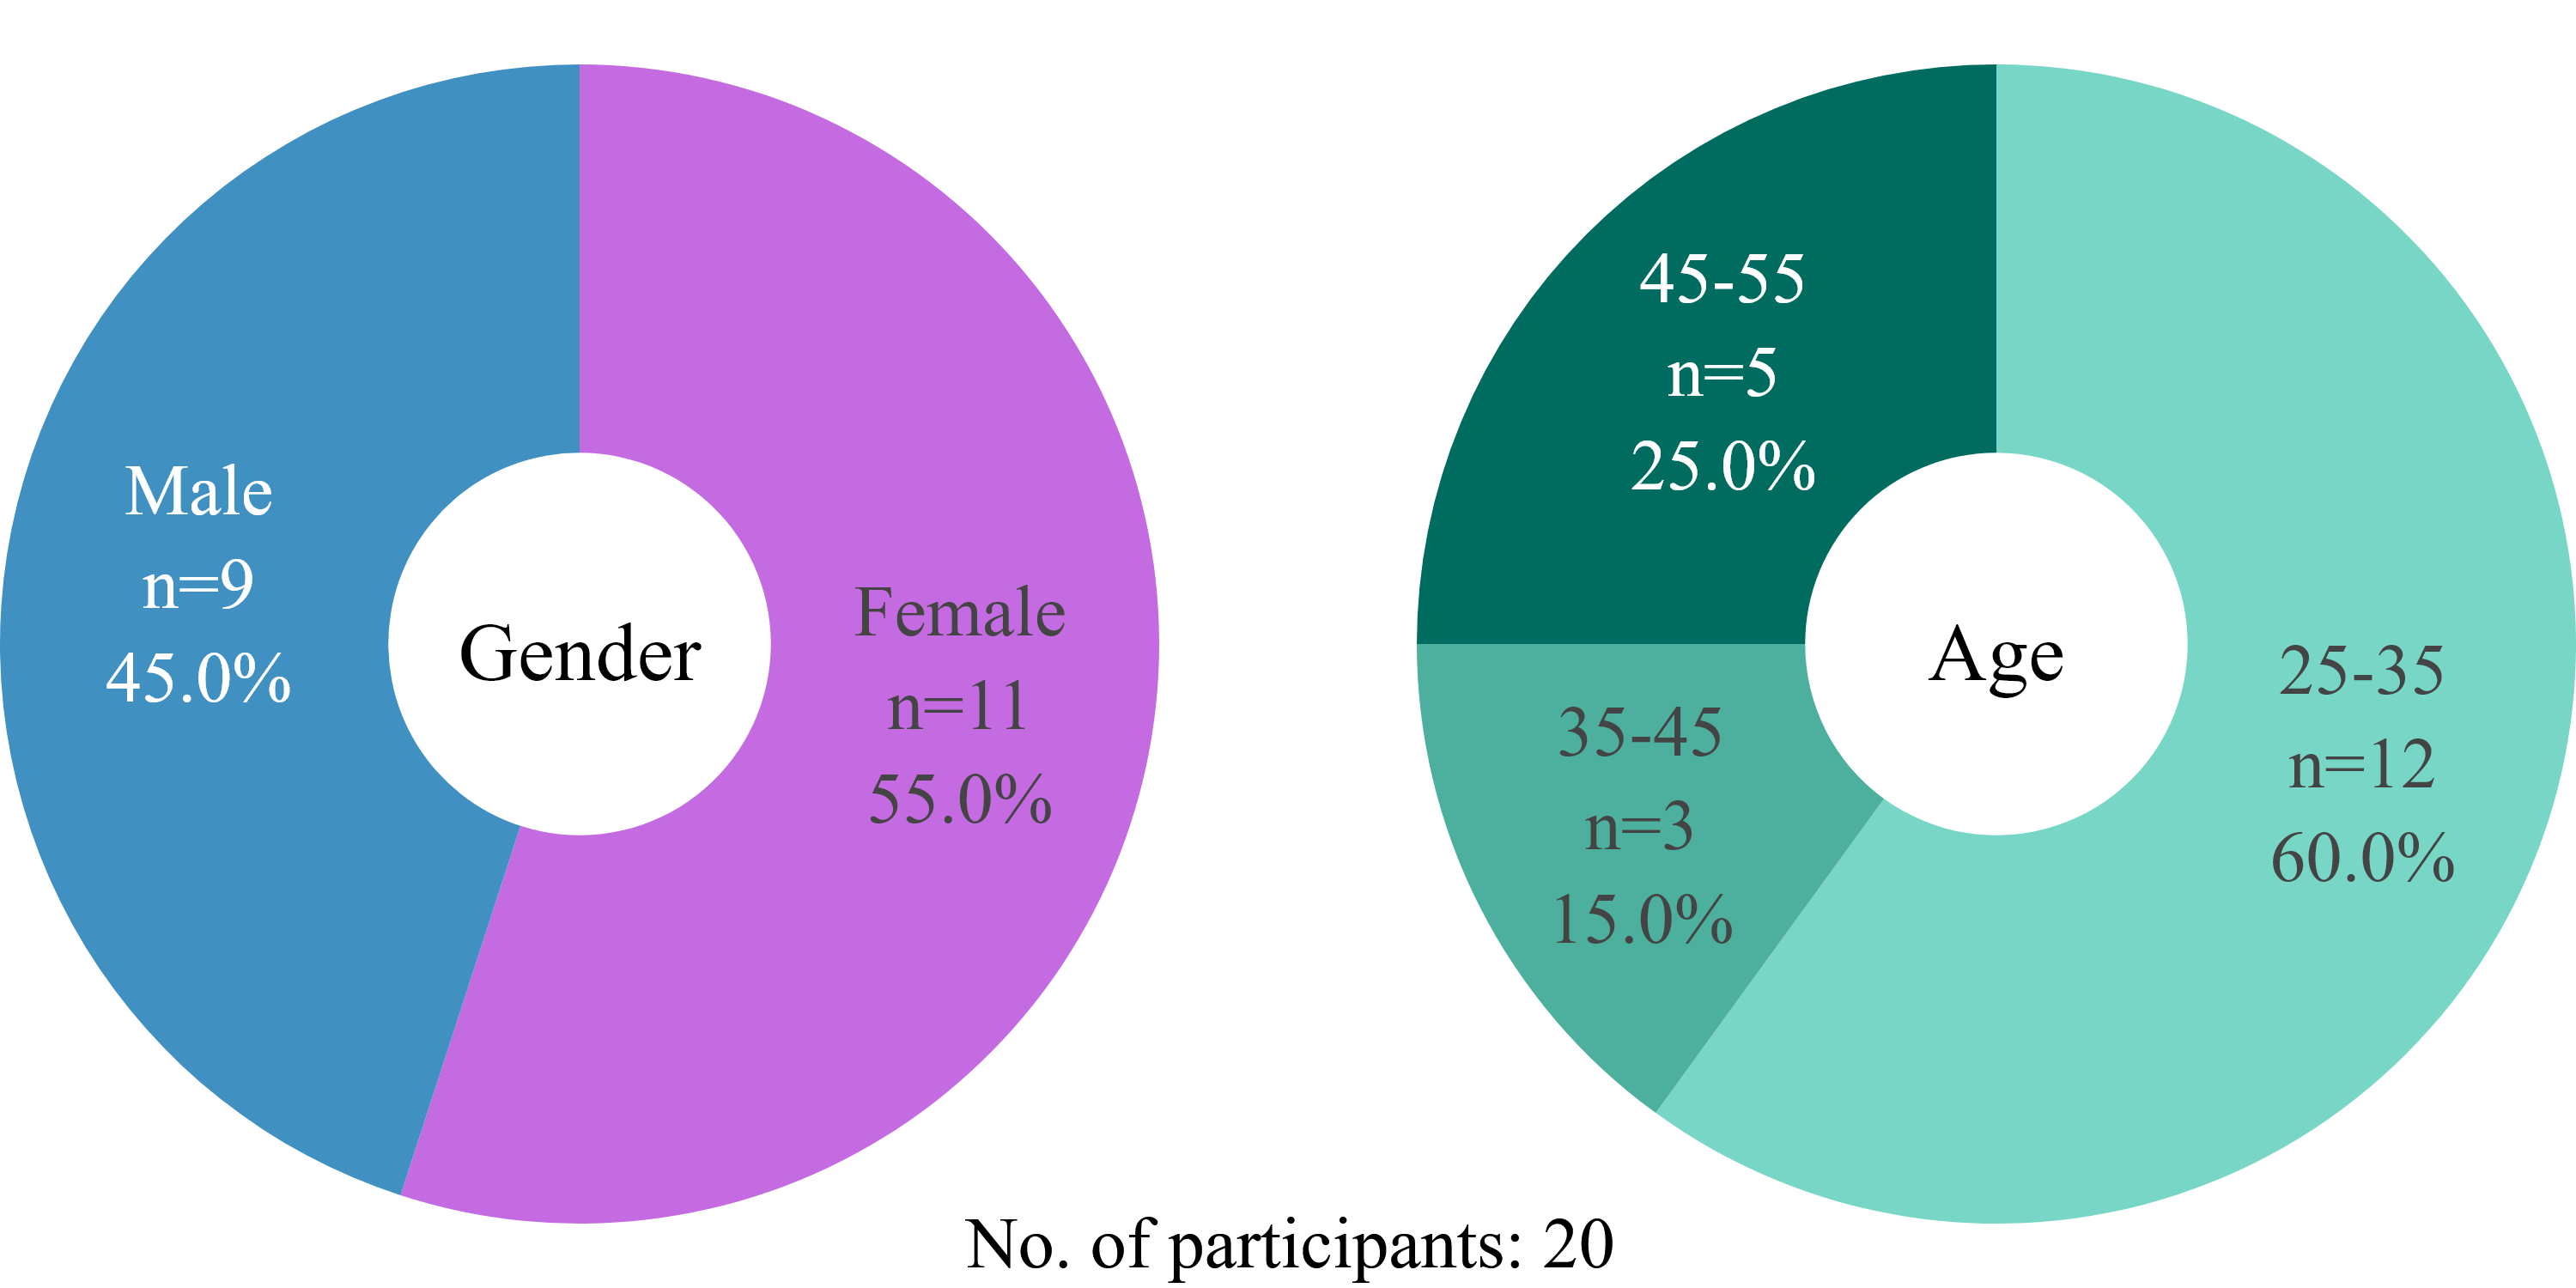
\includegraphics[width=\linewidth]{../demographics_hu}
  \caption{Demographics of the Hungarian participants.}
  \label{fig:demographics_hu}
\end{figure}

\section{Mandarin Chinese survey}

\subsubsection{Materials}

The Chinese survey also contained 50 items with commonly occurring job titles in Mandarin Chinese (Simplified), also in random order. There were six attention checks included to ensure participant engagement and data quality, these were \textit{妈妈} `mother', \textit{爸爸} `father', \textit{女作家} `female writer', \textit{男作家} `male writer', \textit{女画家} `female painter', \textit{男画家} `male painter'. Similarly to the Hungarian attention checks, these words are inherently feminine or masculine in meaning, or explicitly determine gender by prepending 女 `woman' and 男 `man', helping to filter out inattentive responses.

% Say something about Chinese unmarked job titles?

\subsection{Procedure}

Ask Wenhui about the procedure for the Chinese survey.

\subsection{Participants}

The Chinese survey was completed by 24 native Mandarin Chinese speakers, and none of them were rejected after validation. Participants were paid a small fee for completing the questionnaire. The 24 participants (10 female, 14 male) were mostly university students, aged <25 (n=15), 25-35 (n=8), or 35-45 (n=1). See Figure~\ref{fig:demographics_zh} for the distribution.

\begin{figure}[ht]
  \centering
  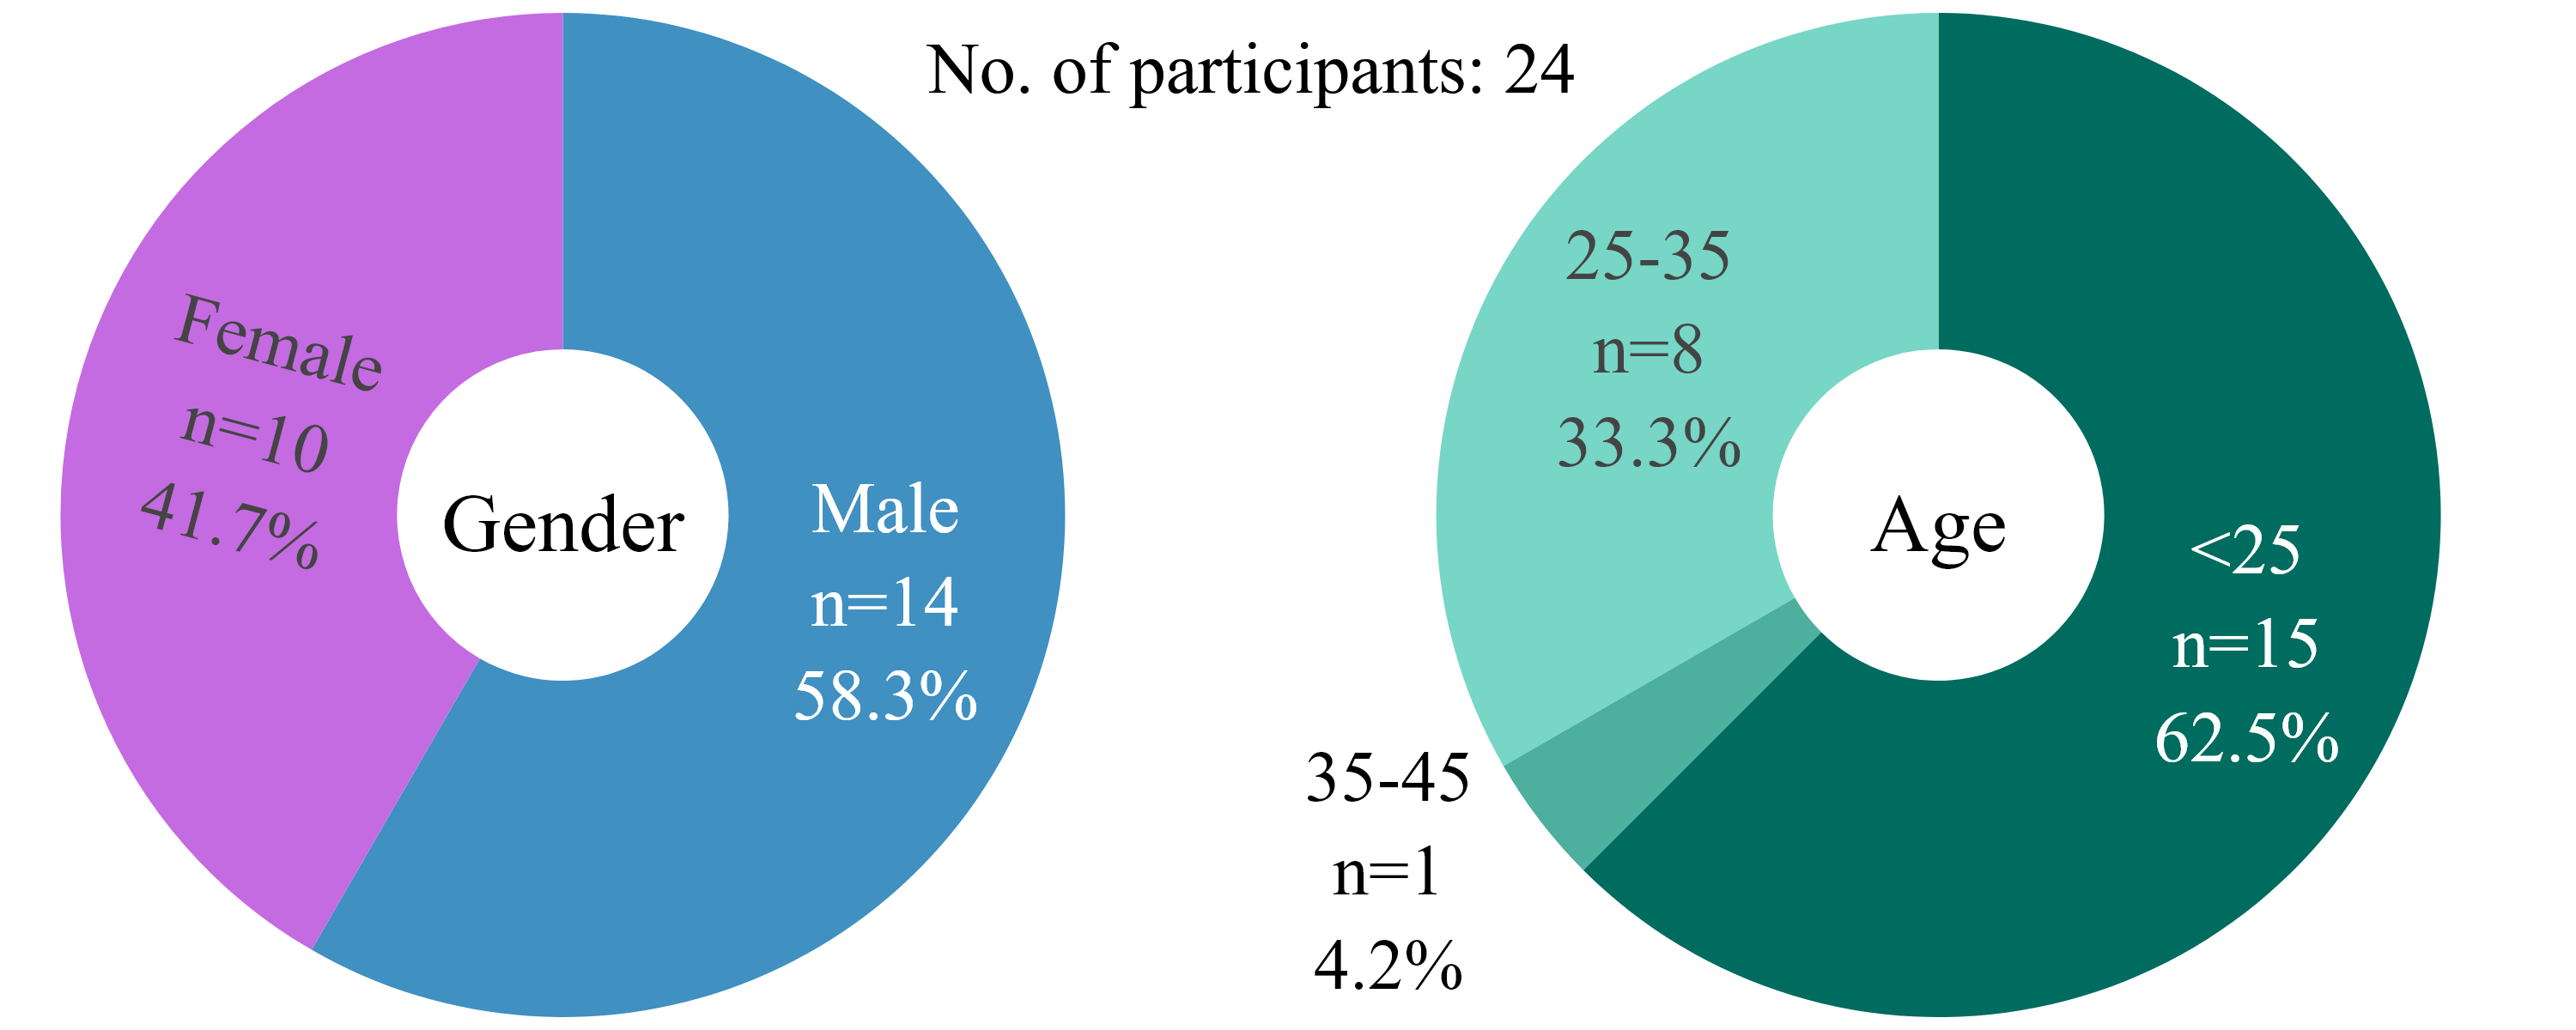
\includegraphics[width=\linewidth]{../demographics_zh}
  \caption{Demographics of the Chinese participants.}
  \label{fig:demographics_zh}
\end{figure}






% ## **2. Methodology (Approx. 0.5 - 0.75 pages)**

% This section should be concise and clear, allowing for replication.

% * **Participants**:
%     * Describe the two groups of participants: 20 Hungarian speakers and 17 Chinese speakers.
%     * Mention key demographics you collected (e.g., for the Hungarian group: 11 female, 9 male, with age ranges of 25-35, 35-45, and 45-55).
% * **Materials**:
%     * State the number of occupational titles rated in each language (44 for Hungarian, 41 for Chinese).
%     * Explain that these were common job titles presented without context. Mention that you also included and then removed attention-check items (e.g., *pincérnő*, *女画家*).
% * **Procedure**:
%     * Describe the rating task: participants rated each occupation on a 7-point Likert scale from -3 (typically male) to +3 (typically female), with 0 representing neutrality.
%     * Mention the platform used for data collection (e.g., Prolific for the Hungarian data).
% * **Data Analysis**:
%     * Briefly state the statistical tests used:
%         * **One-sample t-tests** to determine if the mean rating for each occupation was significantly different from 0 (neutral).
%         * **Independent samples t-tests** to compare ratings between different groups (male vs. female participants for the Hungarian data, and Hungarian vs. Chinese participants for common occupations).
%     * Mention the significance level (p < 0.05).

% ---


% %%%%%%%%%%%%%%%%%%%%%%%%%%%%%%%%%%%%%%%%%%%%%%%%%%%%%%%%%%%%%%%

% ## **Paper Outline**

% ### **1. Introduction (Approx. 0.5 pages)**

% * **Hook**: Start by highlighting the persistence of gender stereotypes in professional life, even as societies strive for equality.
% * **Background**: Briefly discuss the role of language in shaping and reflecting social biases. Introduce the concept of grammatical gender and how its absence in languages like Hungarian and Chinese makes them interesting case studies. The central question is: *How are gender stereotypes encoded and perpetuated without grammatical gender?*
% * **Research Questions**: Clearly state your research questions. For example:
%     1.  To what extent do speakers of Hungarian and Chinese exhibit gender bias when rating occupations?
%     2.  Are there significant differences in gender bias between male and female raters within the same language?
%     3.  What are the key differences and similarities in occupational gender stereotypes between Hungarian and Chinese speakers?
% * **Hypothesis (Optional but Recommended)**: You might hypothesize that despite the lack of grammatical gender, significant gender stereotypes will be present in both languages, potentially reflecting cultural rather than purely linguistic norms.
% * **Roadmap**: Briefly outline the structure of your paper.

% ---

\section{Results \& Analysis}

...overall...

\subsection{Hungarian}

The Hungarian data was first analyzed using a one-sample \textit{t}-test to determine which of the occupations showed a significant bias measured from 0 (neutral/equal). The results showed that the majority of occupational titles (36 out of 44) were rated with a significant gender bias. See Figure \ref{fig:occupations_hu} for a visualization of the mean ratings.

Occupations were rated according to expectations, following societal stereotypes. Words with the highest female bias were \textit{nővér} `nurse' (2.20), \textit{kozmetikus} `beautician' (2.20), \textit{házvezető} `housekeeper' (1.80), \textit{légiutas-kísérő} `flight attendant' (1.40), and \textit{takarító} `cleaner' (1.25), while words with the highest male bias included \textit{munkás} `worker' (-1.40), \textit{pilóta} `pilot' (-1.65), \textit{katona} `soldier' (-1.80), \textit{biztonsági őr} `security guard' (-1.90), and \textit{tűzoltó} `firefighter' (-2.20).

The 8 job titles that came back as not significantly biased were: \textit{ápoló} `nurse' (0.45), \textit{PR mukatárs} `PR worker' (0.30), \textit{felszolgáló} `server' 0.20, \textit{jegyárus} `ticket seller' (0.20), \textit{diák} `student' (0), \textit{tanár} `teacher' (0), \textit{bíró} `judge' (-0.25), and \textit{titkár} `secretary' (-0.30). It is worth noting that while \textit{diák} `student' was rated 0 by absolutely everyone, \textit{tanár} `teacher' had more variety in the ratings, with a high standard deviation.

The strongest agreement were on \textit{diák} `student' (0), \textit{bíró} `judge' (-0.25), \textit{biztonsági őr} `security guard' (-1.90), \textit{tudós} `scientist' (-0.40), and \textit{orvos} `doctor' (-0.55).

\begin{figure*}[ht]
  \centering
  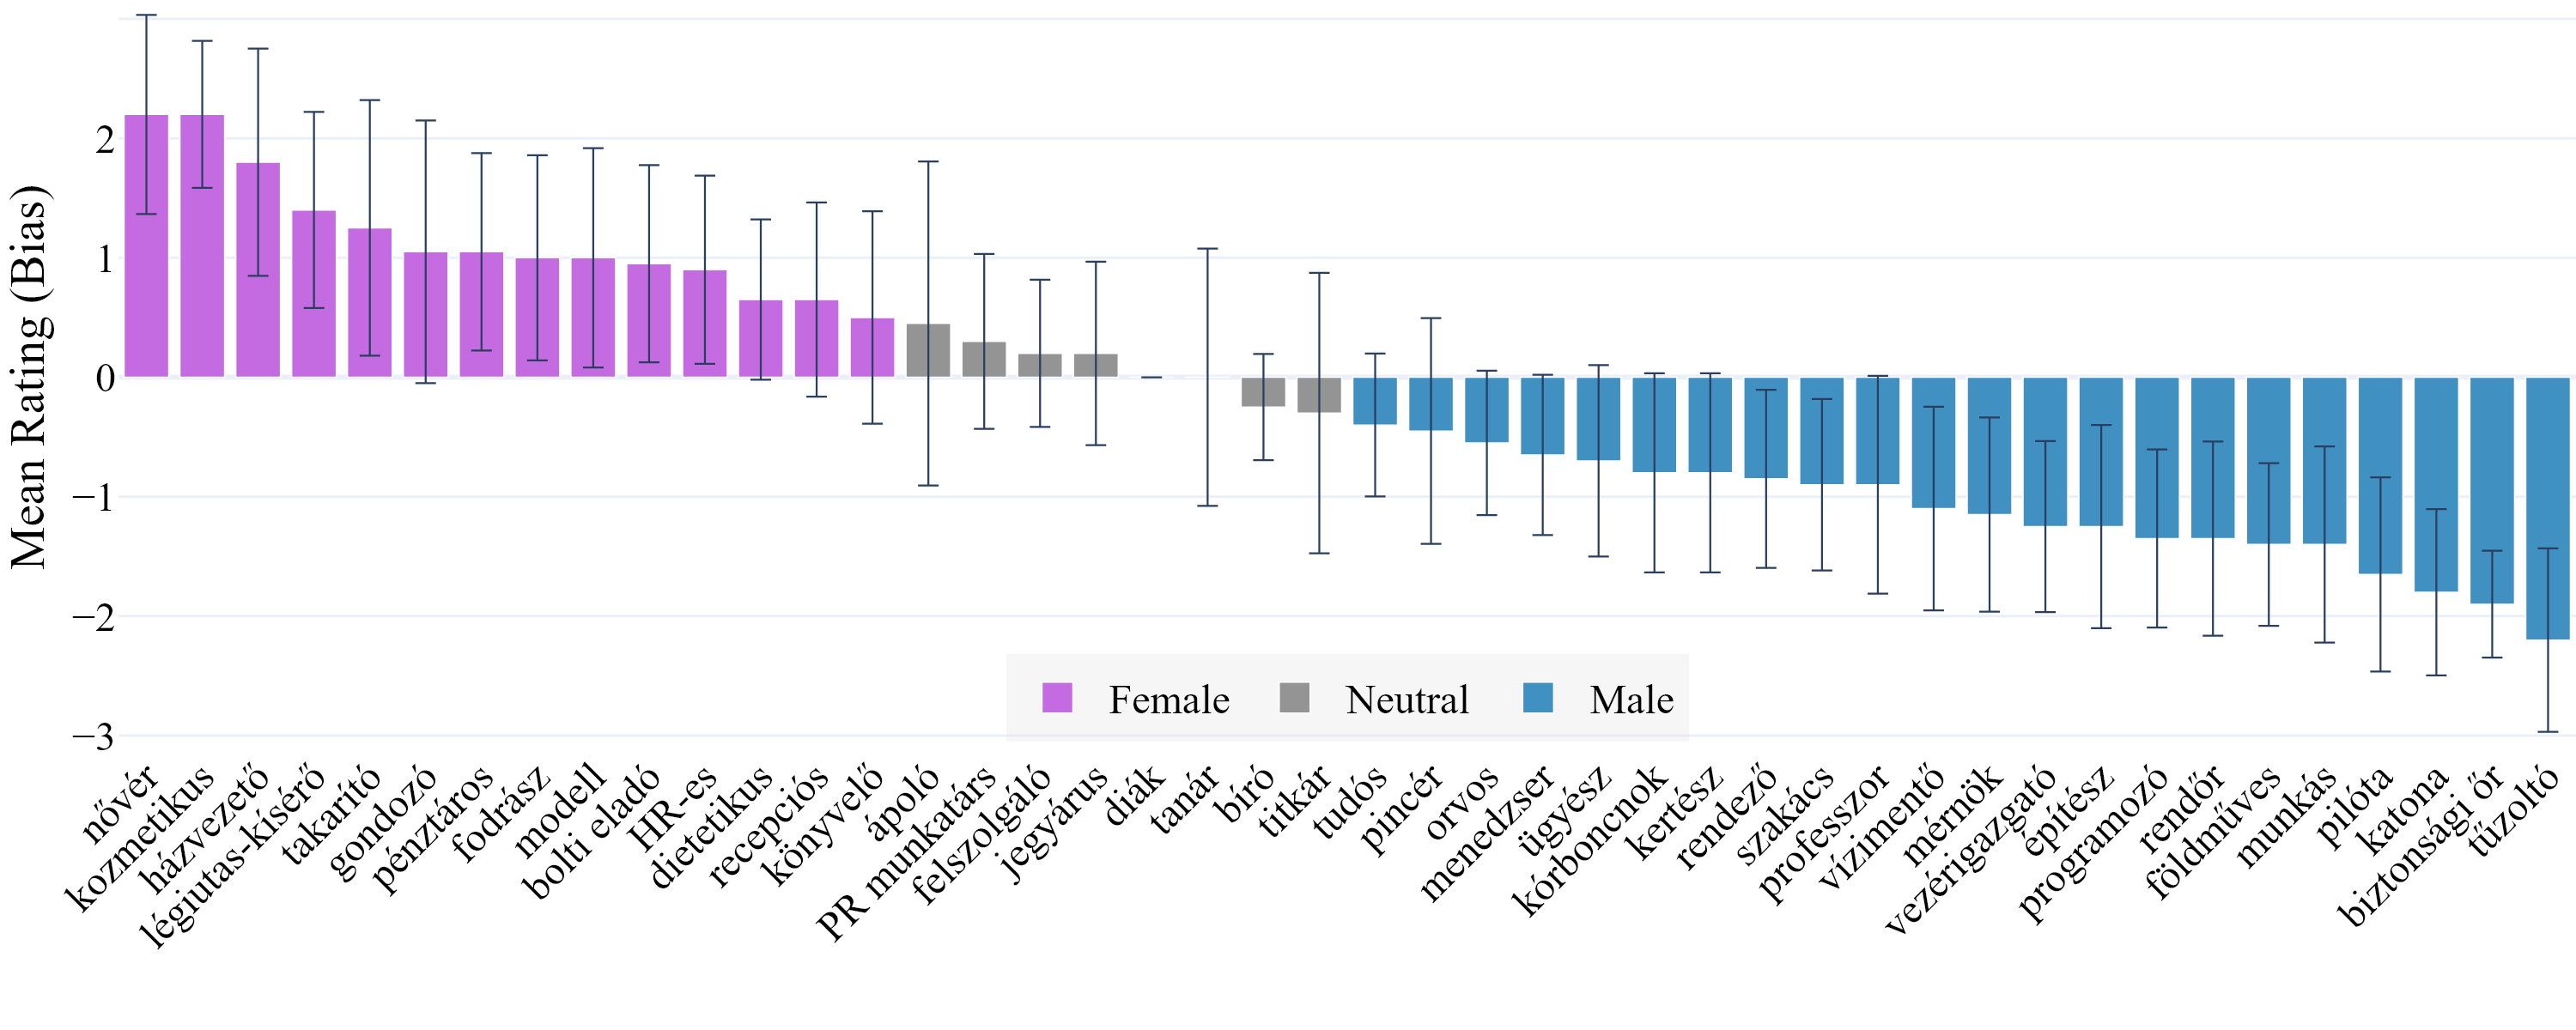
\includegraphics[width=\linewidth]{../occupations_hu}
  \caption{Mean ratings of occupational titles in Hungarian with standard deviations, significant gender bias highlighted -- \href{https://htmlpreview.github.io/?https://github.com/partigabor/occupational-bias/blob/main/occupations_hu.html}{explore the interactive plot}.}
  \label{fig:occupations_hu}
\end{figure*}

LLMs?

We also ran a two-sample \textit{t}-test to compare the ratings of male and female participants for each occupation, and see if there was any significant difference between the two groups. The only job that showed a significant difference was \textit{rendőr} `police', where the male bias was much higher by male raters (-1.77 vs. -1.00). The results are summarized in Figure \ref{fig:occupations_hu_gender}.

\begin{figure*}[ht]
  \centering
  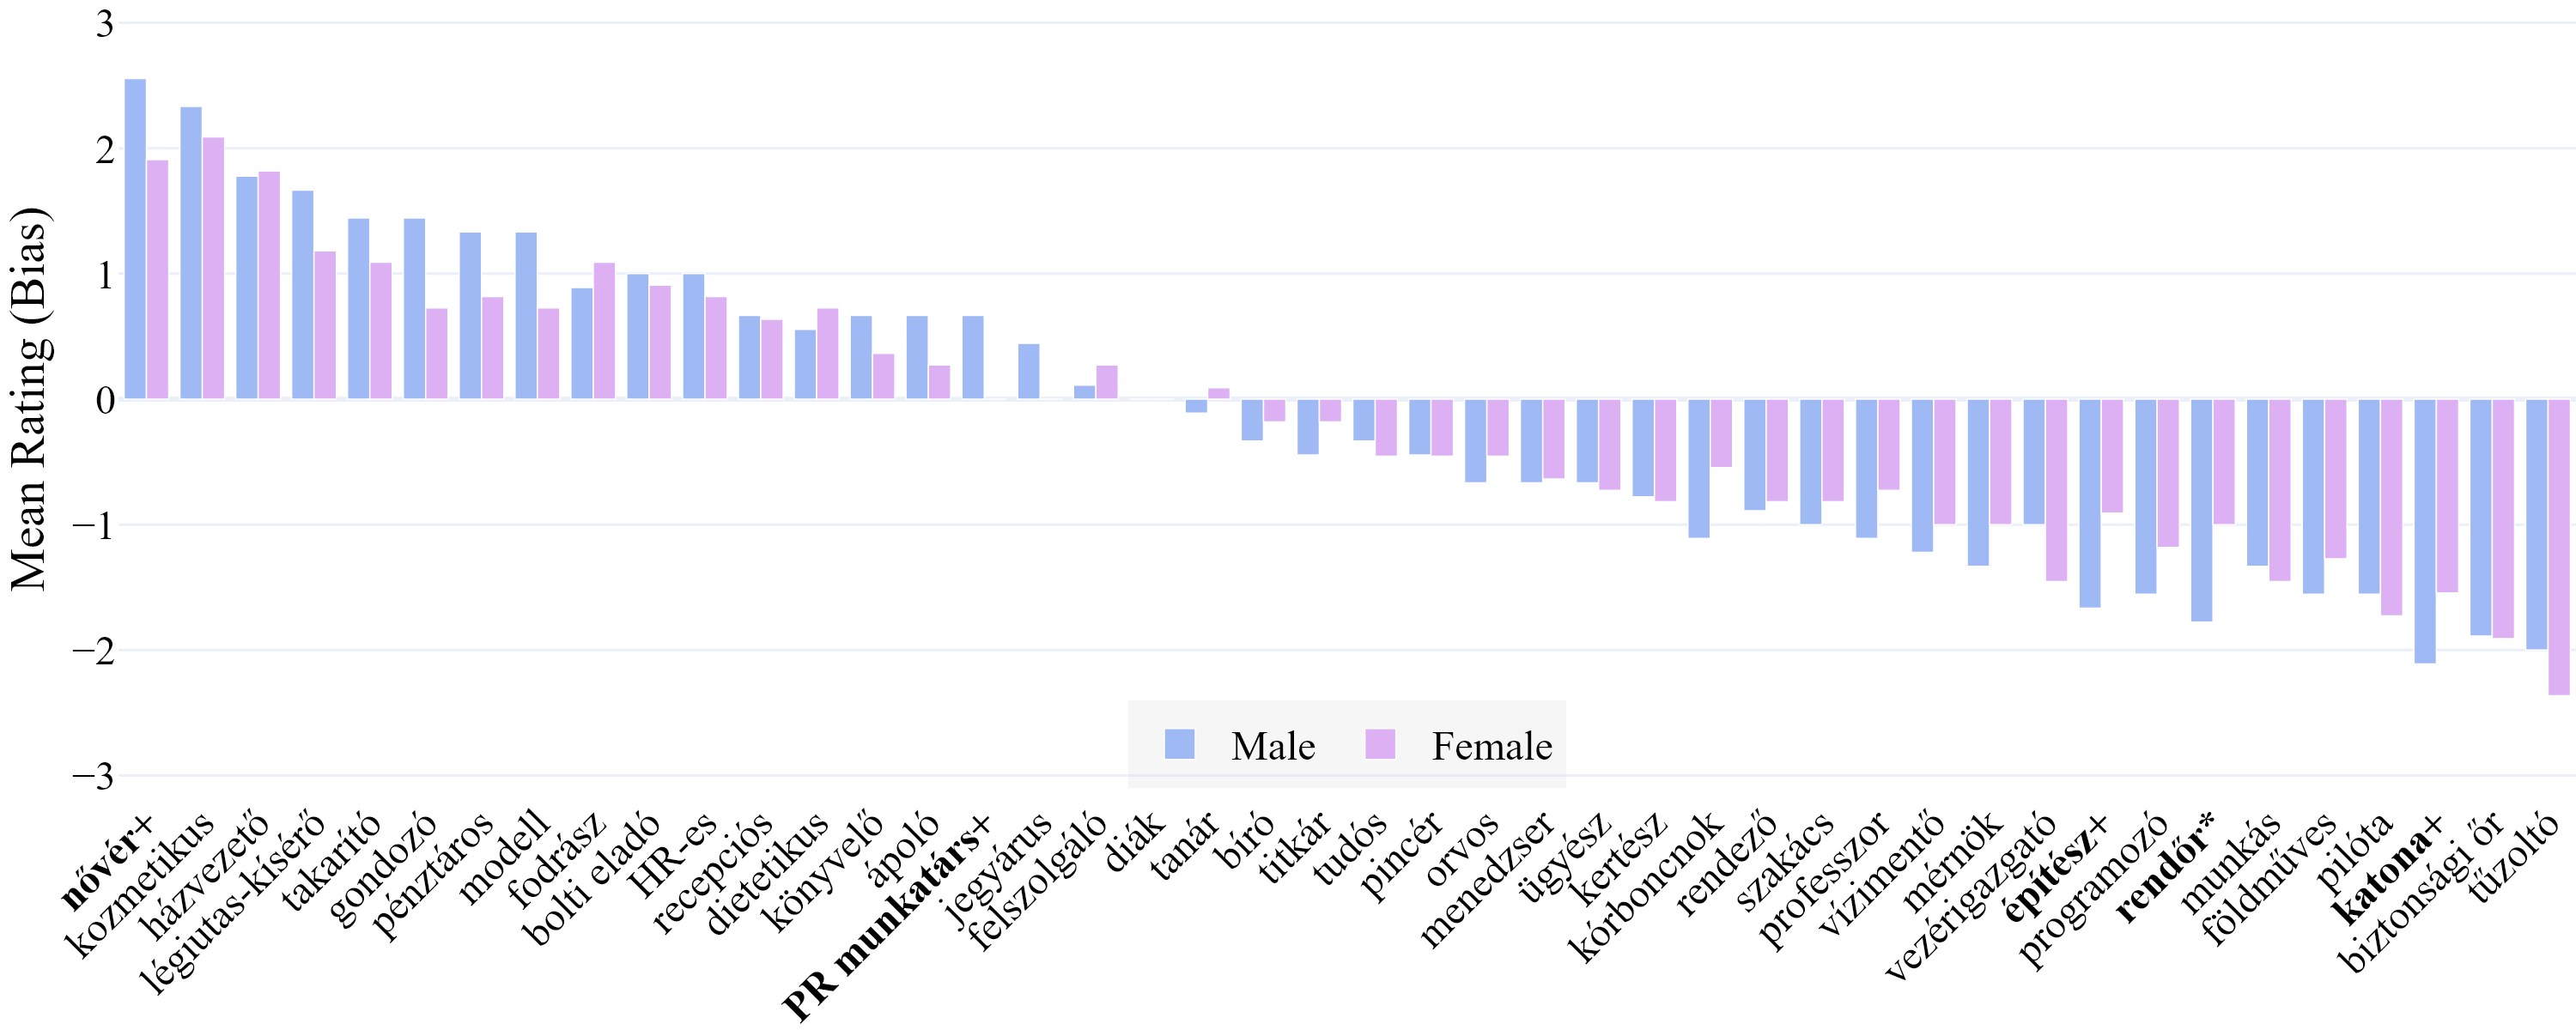
\includegraphics[width=\linewidth]{../occupations_hu_gender}
  \caption{Mean ratings of occupational titles in Hungarian by gender, significant differences highlighted (significant*, and marginally significant+ in \textbf{bold}) -- \href{https://htmlpreview.github.io/?https://github.com/partigabor/occupational-bias/blob/main/occupations_hu_gender.html}{explore the interactive plot}.}
  \label{fig:occupations_hu_gender}
\end{figure*}

\subsection{Chinese}

Similarly to Hungarian, we found that a majority of occupations in Chinese were also rated with significant gender bias. The results of the one-sample \textit{t}-test showed that 40 out of 44 occupations were biased, with only \textit{学生} `student' showing no significant bias.

\subsection{Cross-linguistic comparison}

We compared the ratings of the \hl{42 common items} in the two datasets, again, using a two-sample \textit{t}-test to see if there were significant differences between the two languages. The results are summarized in Figure \ref{fig:occupations_comparison}. Explain...

\begin{figure*}[ht]
  \centering
  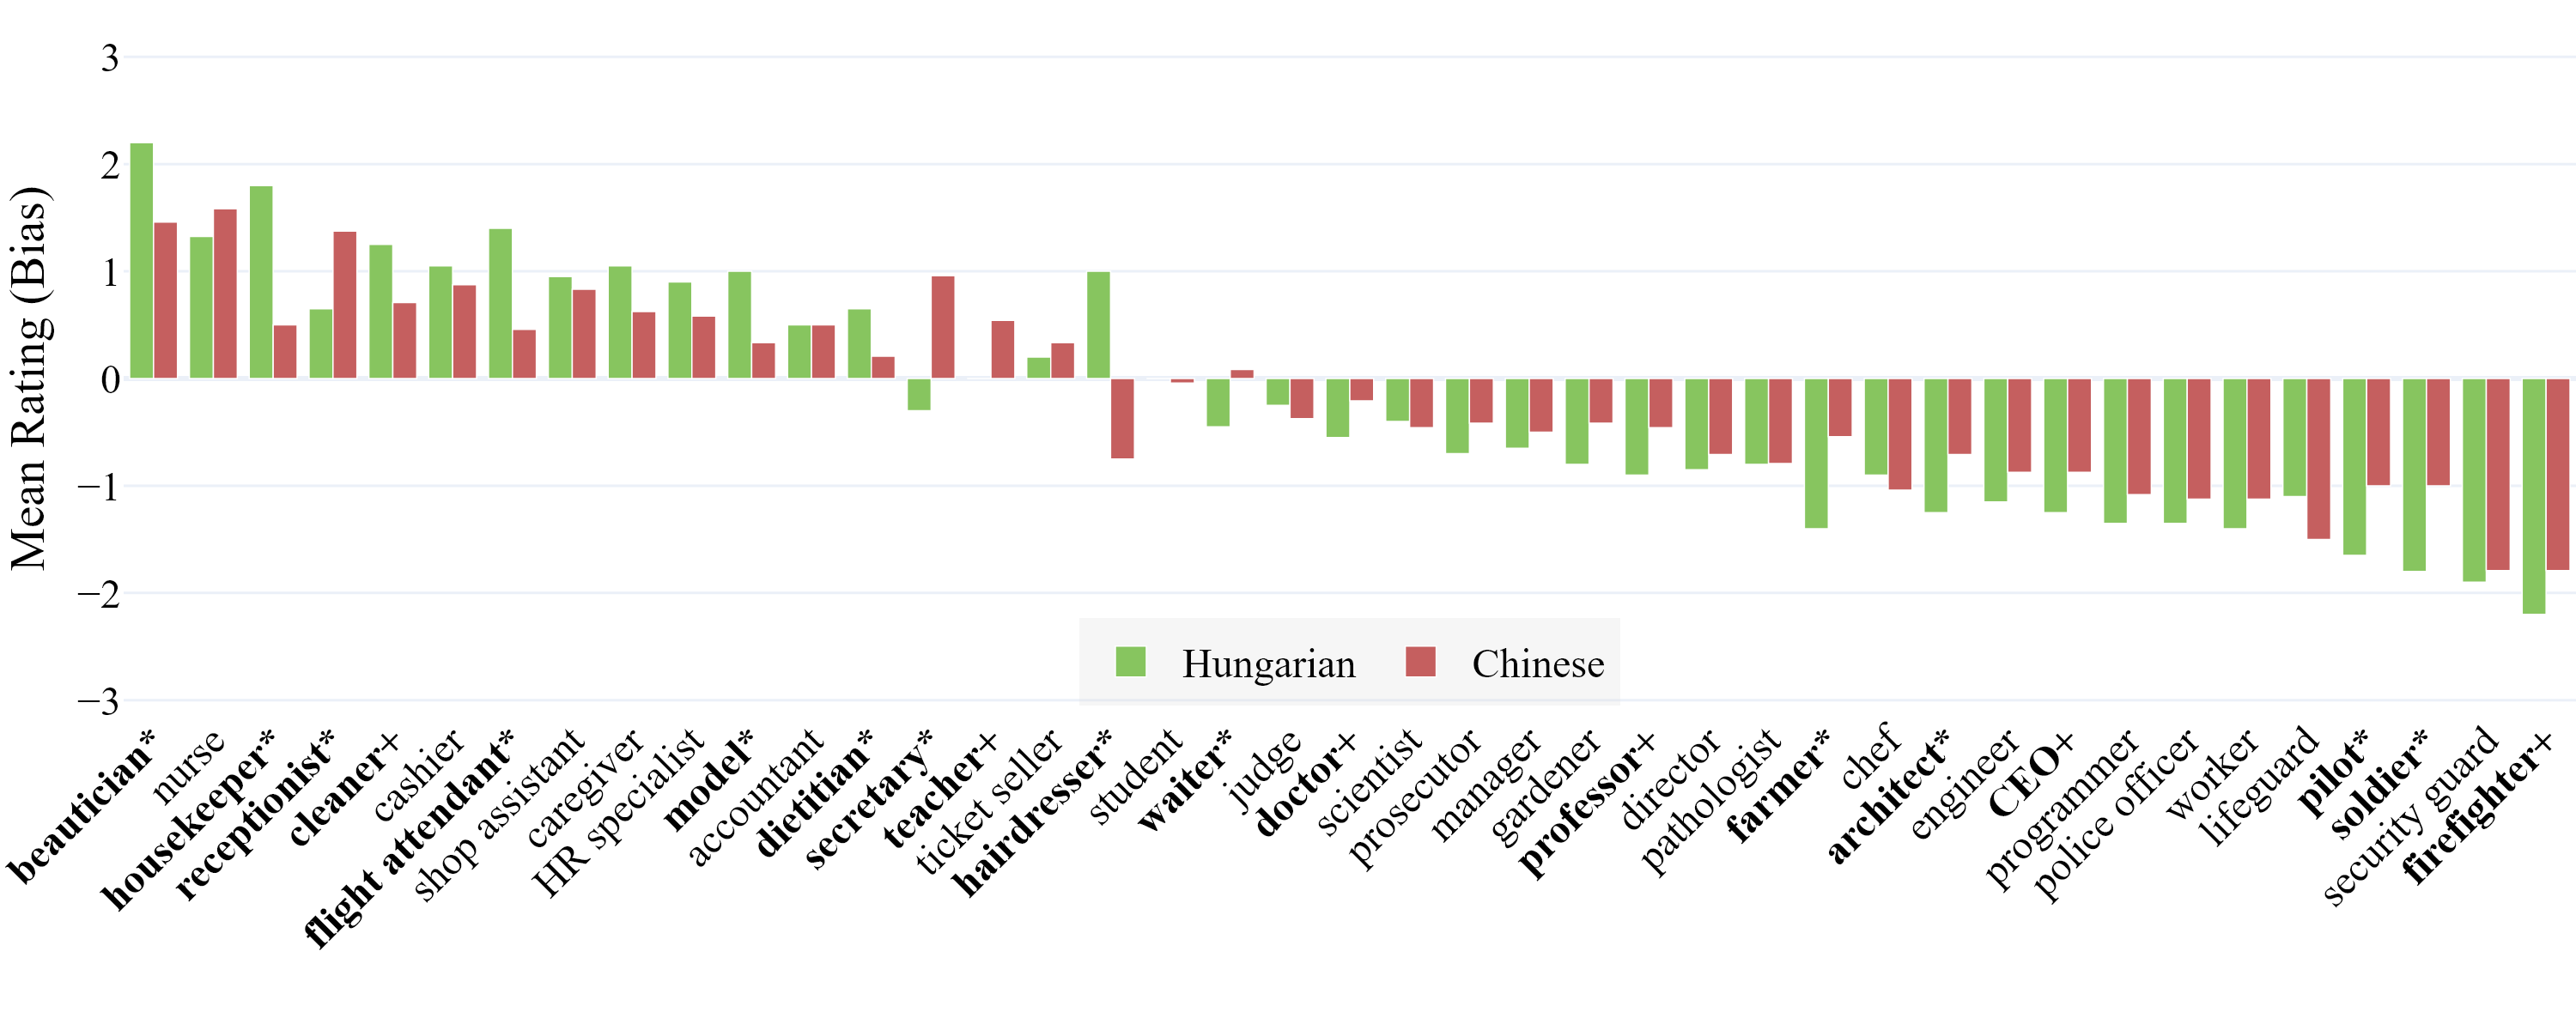
\includegraphics[width=\linewidth]{../occupations_comparison}
  \caption{Mean ratings of common occupational titles in Hungarian and Chinese, significant differences highlighted (significant*, and marginally significant+ in \textbf{bold}) -- \href{https://htmlpreview.github.io/?https://github.com/partigabor/occupational-bias/blob/main/occupations_comparison.html}{explore the interactive plot}.}
  \label{fig:occupations_comparison}
\end{figure*}



% ## **3. Results (Approx. 1 - 1.25 pages)**

% Present your findings clearly. You can integrate one or two key figures here.

% * **Overall Bias**:
%     * Report that a majority of occupations were rated with a significant gender bias in both languages. Reference your one-sample t-test results. For example, in Hungarian, 37 out of 44 occupations showed significant bias, and in Chinese, 39 out of 40 were biased.
% * **Intra-language Gender Differences (Hungarian Data)**:
%     * Summarize the findings of the t-tests comparing male and female participants. Your bar chart (*occupations\_gender\_ttest\_hu.png*) is perfect for this. Highlight any occupations where men's and women's ratings were significantly different (e.g., *építész*, *rendőr*).
%     * Your confusion matrix also offers a neat summary, showing that men's ratings tended to have a greater absolute bias for both male- and female-coded jobs.
% * **Cross-Linguistic Comparison**:
%     * This is a core part of your paper. Use your comparative bar chart (*occupations\_comparison\_ttest.png*).
%     * Focus on the most interesting findings from the t-tests comparing Hungarian and Chinese ratings for the 37 common occupations.
%     * **Highlight major differences**: The most striking is **"hairdresser"** (*fodrász* vs. *理发师*), which shows a strong female bias in Hungarian (+0.95) and a strong male bias in Chinese (-1.06). This is a great example to discuss.
%     * **Point out similarities**: Mention occupations that are strongly biased in the same direction in both cultures, such as "nurse" (female-biased) and "firefighter" (male-biased).
% * **Comparison with Large Language Models (LLMs)**:
%     * Briefly introduce the data from ChatGPT, Gemini, etc., as a point of comparison. You can include the *occupations_hu_llms.png* or *occupations_zh_llms.png* plot.
%     * Note how the LLMs often show even stronger biases than human participants, and their ratings align with the general trends observed in the human data. This adds a modern, impactful layer to your paper.

% ---

% ## **4. Discussion (Approx. 1 page)**

% This is where you interpret your results and highlight the importance of your study.

% * **Summary of Findings**: Briefly restate your main findings.
% * **Gender Bias in Ungendered Languages**: Discuss the key takeaway: the absence of grammatical gender does not prevent strong gender stereotypes from being encoded in language and cognition. The bias is likely rooted in societal structures, cultural norms, and extralinguistic context, which are then reflected in word associations.
% * **Cultural Specificity**: Use your cross-linguistic findings to argue for the cultural specificity of some stereotypes. The "hairdresser" example is your strongest evidence here. You can speculate on the cultural reasons for this difference.
% * **The Role of Participant Gender**: Discuss why male and female participants might rate occupations differently. This could relate to personal experience, societal expectations, or in-group/out-group perceptions.
% * **Implications and Future Directions**:
%     * What are the real-world implications of these biases (e.g., in career counseling, job advertisements, AI applications)?
%     * Your comparison with LLMs is highly relevant here. It shows that these societal biases are being learned and potentially amplified by AI systems.
%     * Suggest future research: expanding the list of occupations, including more languages, or using different methodologies (e.g., implicit association tests).
% * **Limitations**: Briefly acknowledge the limitations of your study (e.g., small sample sizes, the specific set of occupations chosen).

% ---

% ## **5. Conclusion (1-2 paragraphs)**

% * Concisely summarize the study's contribution: it provides empirical evidence of occupational gender bias in Hungarian and Chinese, highlighting both universal and culture-specific stereotypes. Reiterate that these biases persist strongly even in the absence of grammatical gender.

% ---

% %%%%%%%%%%%%%%%%%%%%%%%%%%%%%%%%%%%%%%%%%%%%%%%%



\section{Experiment design}



% \section{Introduction}

% These instructions are for authors submitting papers to *ACL conferences using \LaTeX. They are not self-contained. All authors must follow the general instructions for *ACL proceedings,\footnote{\url{http://acl-org.github.io/ACLPUB/formatting.html}} and this document contains additional instructions for the \LaTeX{} style files.

% The templates include the \LaTeX{} source of this document (\texttt{acl\_latex.tex}),
% the \LaTeX{} style file used to format it (\texttt{acl.sty}),
% an ACL bibliography style (\texttt{acl\_natbib.bst}),
% an example bibliography (\texttt{custom.bib}),
% and the bibliography for the ACL Anthology (\texttt{anthology.bib}).

% \section{Engines}

% To produce a PDF file, pdf\LaTeX{} is strongly recommended (over original \LaTeX{} plus dvips+ps2pdf or dvipdf).
% The style file \texttt{acl.sty} can also be used with
% lua\LaTeX{} and
% Xe\LaTeX{}, which are especially suitable for text in non-Latin scripts.
% The file \texttt{acl\_lualatex.tex} in this repository provides
% an example of how to use \texttt{acl.sty} with either
% lua\LaTeX{} or
% Xe\LaTeX{}.

% \section{Preamble}

% The first line of the file must be
% \begin{quote}
% \begin{verbatim}
% \documentclass[11pt]{article}
% \end{verbatim}
% \end{quote}

% To load the style file in the review version:
% \begin{quote}
% \begin{verbatim}
% \usepackage[review]{acl}
% \end{verbatim}
% \end{quote}
% For the final version, omit the \verb|review| option:
% \begin{quote}
% \begin{verbatim}
% \usepackage{acl}
% \end{verbatim}
% \end{quote}

% To use Times Roman, put the following in the preamble:
% \begin{quote}
% \begin{verbatim}
% \usepackage{times}
% \end{verbatim}
% \end{quote}
% (Alternatives like txfonts or newtx are also acceptable.)

% Please see the \LaTeX{} source of this document for comments on other packages that may be useful.

% Set the title and author using \verb|\title| and \verb|\author|. Within the author list, format multiple authors using \verb|\and| and \verb|\And| and \verb|\AND|; please see the \LaTeX{} source for examples.

% By default, the box containing the title and author names is set to the minimum of 5 cm. If you need more space, include the following in the preamble:
% \begin{quote}
% \begin{verbatim}
% \setlength\titlebox{<dim>}
% \end{verbatim}
% \end{quote}
% where \verb|<dim>| is replaced with a length. Do not set this length smaller than 5 cm.

% \section{Document Body}

% \subsection{Footnotes}

% Footnotes are inserted with the \verb|\footnote| command.\footnote{This is a footnote.}

% \subsection{Tables and figures}

% See Table~\ref{tab:accents} for an example of a table and its caption.
% \textbf{Do not override the default caption sizes.}

% \begin{table}
%   \centering
%   \begin{tabular}{lc}
%     \hline
%     \textbf{Command} & \textbf{Output} \\
%     \hline
%     \verb|{\"a}|     & {\"a}           \\
%     \verb|{\^e}|     & {\^e}           \\
%     \verb|{\`i}|     & {\`i}           \\
%     \verb|{\.I}|     & {\.I}           \\
%     \verb|{\o}|      & {\o}            \\
%     \verb|{\'u}|     & {\'u}           \\
%     \verb|{\aa}|     & {\aa}           \\\hline
%   \end{tabular}
%   \begin{tabular}{lc}
%     \hline
%     \textbf{Command} & \textbf{Output} \\
%     \hline
%     \verb|{\c c}|    & {\c c}          \\
%     \verb|{\u g}|    & {\u g}          \\
%     \verb|{\l}|      & {\l}            \\
%     \verb|{\~n}|     & {\~n}           \\
%     \verb|{\H o}|    & {\H o}          \\
%     \verb|{\v r}|    & {\v r}          \\
%     \verb|{\ss}|     & {\ss}           \\
%     \hline
%   \end{tabular}
%   \caption{Example commands for accented characters, to be used in, \emph{e.g.}, Bib\TeX{} entries.}
%   \label{tab:accents}
% \end{table}

% As much as possible, fonts in figures should conform
% to the document fonts. See Figure~\ref{fig:experiments} for an example of a figure and its caption.

% Using the \verb|graphicx| package graphics files can be included within figure
% environment at an appropriate point within the text.
% The \verb|graphicx| package supports various optional arguments to control the
% appearance of the figure.
% You must include it explicitly in the \LaTeX{} preamble (after the
% \verb|\documentclass| declaration and before \verb|\begin{document}|) using
% \verb|\usepackage{graphicx}|.

% \begin{figure}[t]
%   \includegraphics[width=\columnwidth]{example-image-golden}
%   \caption{A figure with a caption that runs for more than one line.
%     Example image is usually available through the \texttt{mwe} package
%     without even mentioning it in the preamble.}
%   \label{fig:experiments}
% \end{figure}

% \begin{figure*}[t]
%   \includegraphics[width=0.48\linewidth]{example-image-a} \hfill
%   \includegraphics[width=0.48\linewidth]{example-image-b}
%   \caption {A minimal working example to demonstrate how to place
%     two images side-by-side.}
% \end{figure*}

% \subsection{Hyperlinks}

% Users of older versions of \LaTeX{} may encounter the following error during compilation:
% \begin{quote}
% \verb|\pdfendlink| ended up in different nesting level than \verb|\pdfstartlink|.
% \end{quote}
% This happens when pdf\LaTeX{} is used and a citation splits across a page boundary. The best way to fix this is to upgrade \LaTeX{} to 2018-12-01 or later.

% \subsection{Citations}

% \begin{table*}
%   \centering
%   \begin{tabular}{lll}
%     \hline
%     \textbf{Output}           & \textbf{natbib command} & \textbf{ACL only command} \\
%     \hline
%     \citep{Gusfield:97}       & \verb|\citep|           &                           \\
%     \citealp{Gusfield:97}     & \verb|\citealp|         &                           \\
%     \citet{Gusfield:97}       & \verb|\citet|           &                           \\
%     \citeyearpar{Gusfield:97} & \verb|\citeyearpar|     &                           \\
%     \citeposs{Gusfield:97}    &                         & \verb|\citeposs|          \\
%     \hline
%   \end{tabular}
%   \caption{\label{citation-guide}
%     Citation commands supported by the style file.
%     The style is based on the natbib package and supports all natbib citation commands.
%     It also supports commands defined in previous ACL style files for compatibility.
%   }
% \end{table*}

% Table~\ref{citation-guide} shows the syntax supported by the style files.
% We encourage you to use the natbib styles.
% You can use the command \verb|\citet| (cite in text) to get ``author (year)'' citations, like this citation to a paper by \citet{Gusfield:97}.
% You can use the command \verb|\citep| (cite in parentheses) to get ``(author, year)'' citations \citep{Gusfield:97}.
% You can use the command \verb|\citealp| (alternative cite without parentheses) to get ``author, year'' citations, which is useful for using citations within parentheses (e.g. \citealp{Gusfield:97}).

% A possessive citation can be made with the command \verb|\citeposs|.
% This is not a standard natbib command, so it is generally not compatible
% with other style files.

% \subsection{References}

% \nocite{Ando2005,andrew2007scalable,rasooli-tetrault-2015}

% The \LaTeX{} and Bib\TeX{} style files provided roughly follow the American Psychological Association format.
% If your own bib file is named \texttt{custom.bib}, then placing the following before any appendices in your \LaTeX{} file will generate the references section for you:
% \begin{quote}
% \begin{verbatim}
% \bibliography{custom}
% \end{verbatim}
% \end{quote}

% You can obtain the complete ACL Anthology as a Bib\TeX{} file from \url{https://aclweb.org/anthology/anthology.bib.gz}.
% To include both the Anthology and your own .bib file, use the following instead of the above.
% \begin{quote}
% \begin{verbatim}
% \bibliography{anthology,custom}
% \end{verbatim}
% \end{quote}

% Please see Section~\ref{sec:bibtex} for information on preparing Bib\TeX{} files.

% \subsection{Equations}

% An example equation is shown below:
% \begin{equation}
%   \label{eq:example}
%   A = \pi r^2
% \end{equation}

% Labels for equation numbers, sections, subsections, figures and tables
% are all defined with the \verb|\label{label}| command and cross references
% to them are made with the \verb|\ref{label}| command.

% This an example cross-reference to Equation~\ref{eq:example}.

% \subsection{Appendices}

% Use \verb|\appendix| before any appendix section to switch the section numbering over to letters. See Appendix~\ref{sec:appendix} for an example.

% \section{Bib\TeX{} Files}
% \label{sec:bibtex}

% Unicode cannot be used in Bib\TeX{} entries, and some ways of typing special characters can disrupt Bib\TeX's alphabetization. The recommended way of typing special characters is shown in Table~\ref{tab:accents}.

% Please ensure that Bib\TeX{} records contain DOIs or URLs when possible, and for all the ACL materials that you reference.
% Use the \verb|doi| field for DOIs and the \verb|url| field for URLs.
% If a Bib\TeX{} entry has a URL or DOI field, the paper title in the references section will appear as a hyperlink to the paper, using the hyperref \LaTeX{} package.

% \section*{Limitations}

% Since December 2023, a "Limitations" section has been required for all papers submitted to ACL Rolling Review (ARR). This section should be placed at the end of the paper, before the references. The "Limitations" section (along with, optionally, a section for ethical considerations) may be up to one page and will not count toward the final page limit. Note that these files may be used by venues that do not rely on ARR so it is recommended to verify the requirement of a "Limitations" section and other criteria with the venue in question.

% \section*{Acknowledgments}

% This document has been adapted
% by Steven Bethard, Ryan Cotterell and Rui Yan
% from the instructions for earlier ACL and NAACL proceedings, including those for
% ACL 2019 by Douwe Kiela and Ivan Vuli\'{c},
% NAACL 2019 by Stephanie Lukin and Alla Roskovskaya,
% ACL 2018 by Shay Cohen, Kevin Gimpel, and Wei Lu,
% NAACL 2018 by Margaret Mitchell and Stephanie Lukin,
% Bib\TeX{} suggestions for (NA)ACL 2017/2018 from Jason Eisner,
% ACL 2017 by Dan Gildea and Min-Yen Kan,
% NAACL 2017 by Margaret Mitchell,
% ACL 2012 by Maggie Li and Michael White,
% ACL 2010 by Jing-Shin Chang and Philipp Koehn,
% ACL 2008 by Johanna D. Moore, Simone Teufel, James Allan, and Sadaoki Furui,
% ACL 2005 by Hwee Tou Ng and Kemal Oflazer,
% ACL 2002 by Eugene Charniak and Dekang Lin,
% and earlier ACL and EACL formats written by several people, including
% John Chen, Henry S. Thompson and Donald Walker.
% Additional elements were taken from the formatting instructions of the \emph{International Joint Conference on Artificial Intelligence} and the \emph{Conference on Computer Vision and Pattern Recognition}.








% Bibliography entries for the entire Anthology, followed by custom entries
%\bibliography{anthology,custom}
% Custom bibliography entries only
\bibliography{custom}

\appendix

\section{Example Appendix}
\label{sec:appendix}

This is an appendix.

\end{document}
